\chapter{Introduction}
\label{sec:intro}

In this chapter, a brief introduction on electric vehicles and lithium-ion battery packs is made. Exploring the main insights and challenges related to battery pack aging provides manufacturers and researchers with a motivation for designing new methodologies for a reliable estimation of the state of health of a battery pack -- the main contribution of this thesis.

\section{Electric vehicles}
\label{sec:ev}
Mitigating climate change is considered one of the key challenges of our century. With the growing concerns regarding the causes and effects of climate change, global efforts are being made by governments to accelerate clean energy transition and reach net zero emissions \cite{iea_net_zero}. It is estimated that the transport sector accounts for 27\% of the global emissions of greenhouse gases \cite{iea_emissions} and, more specifically, road travel accounts for three-quarters of transport CO2 emissions \cite{iea_transport_emissions}. Research and development towards a greener automotive industry has therefore gained world-wide momentum in recent years. \textbf{Electric vehicles} (EVs) have been widely accepted as a clean and reliable alternative to fossil fuel vehicles, both in private and public transportation sectors, and are expected to quickly take over the market in the upcoming years \cite{eea_report}. It is therefore important to investigate the main technologies that enhance the performances of an EV.

The core component of an electric vehicle is its rechargeable \textbf{battery pack}. It is the heaviest, largest and most expensive component of an EV \cite{heavy_bulky_expensive}. As such, its design is critical in determining the energy efficiency and driving range of an EV. A battery pack is typically made up of many battery cells, connected in parallel and series. \textbf{Lithium-ion battery} (LIB) cells are currently the dominating technology in battery pack design, thanks to favorable properties such as high energy density and efficiency, low memory effects, long cycle life, low self-discharge rate, high charging and discharging rate capability and -- last but not least -- plummeting costs of their composing materials. \cite{li-ion_data_where,li-ion_battery_properties,li-ion_plummeting_costs}. Li-ion battery cells are discussed more in depth in sec. \ref{sec:li-ion}.

\begin{figure}[hbt!]
    \centering
    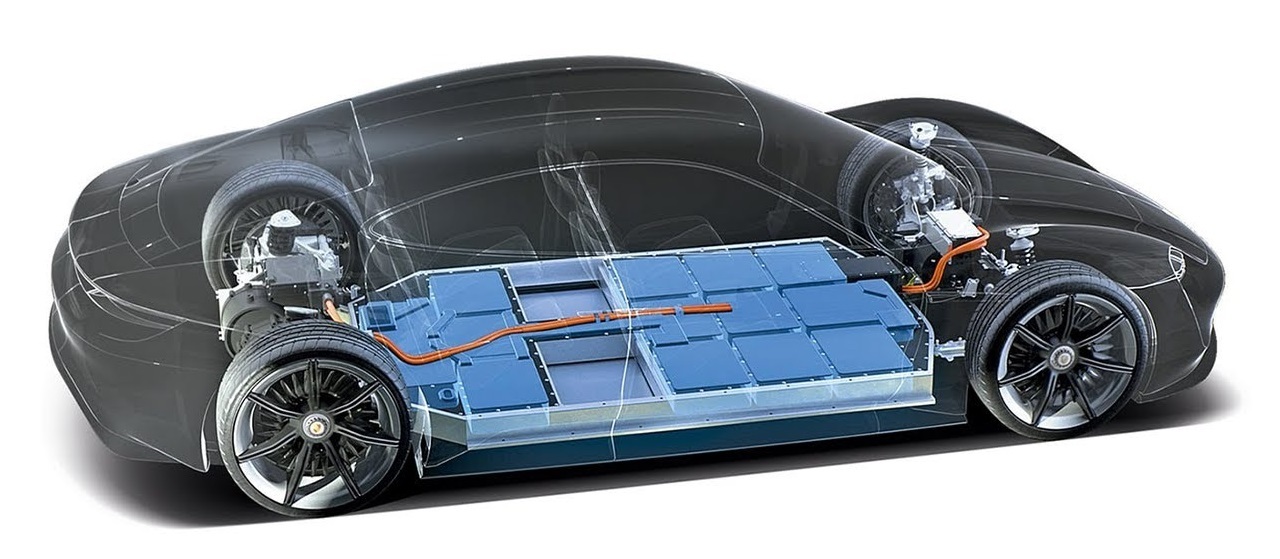
\includegraphics[width=0.9\textwidth]{images/porsche_taycan}
    \caption[An electric car and its battery pack]{An electric car (Porsche Taycan) with its battery pack highlighted. Taken from \cite{porsche_taycan}}
    \label{fig:porsche_taycan}
\end{figure}

A \textbf{battery management system} (BMS) is another important component in the design of an EV \cite{bms}. A BMS is an embedded software system which performs many functions related to the management of a battery pack, such as protecting the battery from operating outside its safe operating area (preventing overcharging and overdischarging, overcurrents, overheating), monitoring its state, calculating and reporting secondary data (such as the remaining driving range), balancing the state of charge among the battery cells and actively managing the battery pack's thermal management system (if present). All these operations are possible because of sensors installed inside the battery pack, which monitor parameters such as terminal voltage, current flow, internal temperature, state of charge and state of health (sec. \ref{sec:soh}) at the cell level. The BMS continuously monitors the sensors' measurements through a communication data bus, commonly known as Controller Area Network (CAN) bus. Moreover, these measurements can be communicated outside the vehicle through an interface called On-Board Diagnostics (OBD) port.

\section{Li-ion battery cell}
\label{sec:li-ion}
EV battery packs are hierarchically structured into three levels: cell, module
and pack \cite{li-ion_battery_properties}.
As visualized schematically in fig. \ref{fig:cell2module2battery}, multiple battery cells are first connected together in series and parallel to form a battery module, and then a certain number of modules are assembled to form a battery pack. This design has the aim of achieving a sufficiently high terminal voltage while adding up the capacity of each individual cell.

\begin{figure}[hbt!]
    \centering
    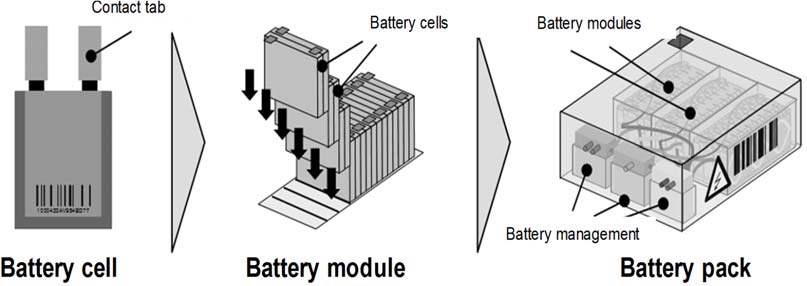
\includegraphics[width=0.8\textwidth]{images/cell2module2battery}
    \caption[From battery cells to a battery pack]{From battery cells to a battery pack. Taken from \cite{cell2module2battery}}
    \label{fig:cell2module2battery}
\end{figure}

Battery cells come in different formats (pouch, cylindrical, prismatic) and chemistries (choice of the anode and cathode materials and electrolyte), which together determine the energy density and efficiency, terminal voltage, safety characteristics, costs, and -- ultimately -- performances. They are typically named according to their cathode materials: for example, lithium-ion battery cells are characterized by lithium-based cathode materials such as lithium cobalt oxide (LiCoO2), lithium iron phosphate (LiFePO4), lithium nickel manganese cobalt oxides (LiNi\textsubscript{x}Mn\textsubscript{y}Co\textsubscript{z}O2, or NMC-xyz for short) and so on \cite{li-ion_chemistries}. Graphite is commonly used as anode material \cite{anode_material}. Cathode and anode are separated by a layer of electrolyte material, which is typically a polymer gel containing lithium salts\footnote{It is worth mentioning that recent advances in battery technology involve using a solid as the electrolyte material, with ceramics being the most promising \cite{solid_electrolyte}. Increased energy density, less need of thermal cooling and improved safety are among the many benefits of using a solid electrolyte.}. The electrolyte has two functions: it prevents the electrical contact between the two electrodes and, at the same time, it allows the diffusion of lithium ions (Li\textsuperscript{+}) from cathode to anode and vice versa.

When a battery is being discharged, Li\textsuperscript{+} ions are shuttled from
the anode to the cathode, forcing electrons to flow around an outside circuit and thus allowing the conversion of chemical energy
into electrical energy (fig. \ref{fig:li-ion_cell}). On the contrary, charging a battery rips Li\textsuperscript{+} ions out of cathode's oxide crystals and pulls them back to the graphite-based anode where they are stored \cite{nature_li-ion}.

\begin{figure}[hbt!]
    \centering
    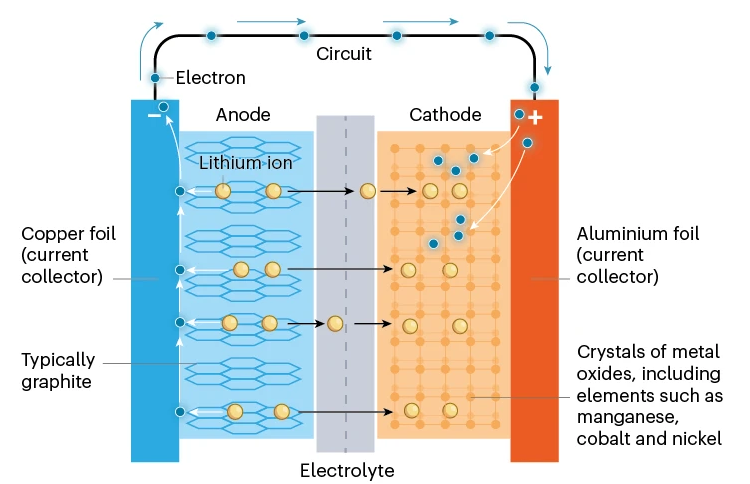
\includegraphics[width=0.8\textwidth]{images/li-ion_cell}
    \caption[Discharging a Li-ion battery cell]{Discharging a Li-ion battery cell. Taken from \cite{nature_li-ion}}
    \label{fig:li-ion_cell}
\end{figure}

\subsection{Battery cell aging and SOH}
\label{sec:soh}
Battery cells are characterized by many parameters describing their electrochemical state and dynamics. The \textbf{capacity} $C$ of a battery is defined as the total amount of charge it can deliver and is commonly measured in ampere-hours [Ah]. Manufacturers usually declare a nominal (or rated) capacity $C_{nominal}$, i.e. the capacity of the battery when it is fresh out of the factory. For instance, a battery rated at 60 Ah can theoretically deliver a current of 5 A for 12 hours. The more electrode material is contained in the cell, the greater is its capacity. Nonetheless, the open-circuit voltage of a battery cell depends solely on its chemistry, regardless of its capacity \cite{battery_glossary}. The ratio between the amount of charge $Q_{available}$ that can be extracted from the battery at a given point in time and the actual capacity $C_{actual}$ is called \textbf{state of charge}:
\begin{equation}
\label{eq:soc}
    SOC = \frac{Q_{available}}{C_{actual}}
\end{equation}

Actually, multiple external factors determine the effective battery capacity $C_{actual}$ at any given moment. Therefore, capacity is typically defined up to a nominal set of operating conditions (or \textbf{nominal conditions}, for short), namely: external temperature equal to room temperature ($\approx 20$ °C) and fixed discharge current magnitude. In fact, capacity tends to increase with high temperatures \cite{C_depends_on_T} and low discharge currents (a phenomenon called Peukert's law \cite{peukert}).

When dealing with a current flowing through a battery, we can also express its magnitude in terms of \textbf{C-rate}. It is defined as the magnitude of the current through the battery divided by the theoretical current draw under which the battery would deliver its capacity in one hour \cite{c-rate}. For instance, when referring to a battery with a capacity of 60 Ah, a current with C-rate 0.5 (or 0.5C current, for short) is a 30 A current.

Li-ion battery cells, like all batteries, are subject to degradation phenomena with time and usage, due to a variety of chemical and mechanical changes to the electrodes. These phenomena gradually lead to a decrease in capacity (a phenomenon called \textbf{capacity fading}) and an increase in internal resistance \cite{capacity_fading}. Other than normal usage in safe operating conditions, common causes of degradation include: shelving a full-charged battery for a long time, overcharging and overdischarging, storage or usage in very hot or very cold environments, high charge/discharge currents, discharging at high deltas of state of charge (depth of discharge, or DOD(\%) for short). There exist a large number of degradation mechanisms\footnote{This list is by no means exhaustive: an in-depth discussion of degradation mechanisms for Li-ion battery cells can be found in \cite{capacity_fading}.}, such as:
\begin{itemize}
    \item thickening of the Solid Electrolyte Interface (SEI), a passivation layer formed on the surface of LIBs' anode material produced by electrolyte decomposition, in which Li\textsuperscript{+} ions get irreversibly trapped (i.e. loss of lithium inventory)
    \item lithium plating, i.e. the deposition of lithium around the anode during charging
    \item loss of cathode and anode material due to its dissolution, cracking, exfoliation, detachment or volume change during usage
    \item corrosion and structural degradation of battery cell components, such as its current collectors.
\end{itemize}

Battery aging can be measured in a variety of ways. The most common way of quantifying the capacity loss of a battery is the \textbf{state of health} (SOH), defined as the ratio of the actual capacity of the battery to its nominal capacity:
\begin{equation}
\label{eq:soh}
SOH = \frac{C_{actual}}{C_{nominal}}
\end{equation}

Another way of expressing the age of a battery is the number of \textbf{equivalent full cycles} (EFC). An EFC is defined as a virtual cycle of charge and discharge of a battery at a specified DOD \cite{efc}. The number of EFCs can be estimated as
\begin{equation}
\label{eq:efc}
EFC = \int \frac{|I|}{2 \cdot DOD \cdot C_{nominal}} \, dt
\end{equation}
where $I$ is the current flowing through the battery. It is easy to observe that the SOH of a battery decreases as the number of EFCs increases; however, there is no general mathematical relationship between the SOH and the number of EFC, as the latter ignores operating conditions such as temperature and C-rate (as opposed to SOH), but also because SOH happens to not decrease uniformly over the lifespan of the battery \cite{efc,efc2}. For instance, at $T=25$ °C and a fixed 0.5C charging and discharging current a battery might undergo 3000 EFC at 100\% DOD before reaching a SOH of 80\%, while at $T=45$ °C and 2C current the same battery might undergo 1200 EFC before reaching 80\% SOH.

\subsection{From cell SOH to pack SOH}
\label{sec:cell_soh2pack_soh}
The cells inside a battery pack are subject to uneven degradation over time, due to their asymmetrical placement inside the pack, uneven temperature distribution, different inter-cell contact resistances and possible subtle differences in their manufacturing quality \cite{uneven_soh}. As a result, each individual cell is characterized by a different capacity and internal resistance. This in turn causes current to flow unevenly among the cells, worsening the imbalance of cell degradation rates. To break this vicious cycle, the BMS tries to balance temperatures and currents inside a battery pack according to the estimated SOH of each cell \cite{bms_balancing1,bms_balancing2}. Due to cell capacity imbalance and the complexity of the BMS, estimating the SOH at the battery pack level in real time is not an easy task.

In the context of EVs, a battery pack is said to be at its \textbf{end of life} (EOL) when its state of health reaches 80\% \cite{eol_def}. This threshold is commonly adopted since below 80\% of its SOH a Li-ion battery pack incurs in a faster, typically more-than-linear degradation \cite{soh_after_eol}.

Monitoring SOH is a critical task, since the EOL of a battery pack typically marks the time when it has to be retired. SOH estimation can be performed in a laboratory setting, but in recent years researchers devoted their efforts to designing real-time and on-board procedures to allow for an easier and cheaper alternative for estimating SOH, as discussed in sec. \ref{sec:aviloo} and chap. \ref{sec:state_of_the_art}.

\section{Proprietary SOH estimation procedures}
\label{sec:aviloo}
Nowadays, a few private EV fleet management companies developed reliable manufacturer-independent, on-board diagnostic procedures for EV battery packs. Typically, they provide such battery tests to customers wishing to assess the degradation of a battery pack before buying or selling an EV.

Such SOH estimation procedures typically consist in connecting a monitoring device to the OBD port of the car and then driving the fully charged vehicle until the SOC drops below 10\%. Meanwhile, the monitoring device continuously collects relevant operating data, which consists of measurements such as voltage, internal and external temperature, current, SOC, power consumption and so on, sampled with a relatively high frequency and possibly at the cell, module and pack level simultaneously. Finally, this data is used as the input of a proprietary SOH prediction algorithm, which provides the customer with a reliable estimate of the SOH of their EV's battery pack.

Some of these companies retain the collected EV field data. This data is invaluable as it can be used for further analyses on the monitored battery, but can also be exploited for research purposes. Indeed, such data is extremely useful in designing data-driven methods to predict the SOH of a battery pack, as discussed throughout this thesis.

%The field data collected during each bcheck can be viewed on a portal called AVILOO Battery Cloud, and consists of measurements such as voltage, internal and external temperature, current, SOC, power consumption and so on, sampled with a relatively high frequency and possibly at the cell, module and pack level simultaneously. EV monitoring data is extremely useful in designing data-driven methods to predict the SOH of a battery pack, as discussed throughout this thesis.


%AVILOO GmbH is an Austrian company born in 2017 with the mission of developing the first manufacturer-independent diagnostic procedure for EV battery packs. According to their website\footnote{ \url{https://aviloo.com/}\label{note:aviloo_website}}, they designed a reliable, on-board SOH estimation procedure with a claimed maximum estimation error of $\pm 1.5\%$. They provide their test to customers typically wishing to assess the degradation of a battery pack before buying or selling an EV.

%AVILOO Battery Test, also called \textbf{bcheck} (short for "battery check"), consists in connecting a monitoring device to the OBD port of the car, and then driving the fully charged vehicle until the SOC drops below 10\%. Meanwhile, the monitoring device continuously collects relevant data and sends it to AVILOO's servers. Then, this data is used as the input of AVILOO's SOH estimation algorithm. The customer finally receives a detailed certificate (fig. \ref{fig:aviloo_certificate}) reporting the estimated SOH value and other valuable information about the tested battery pack.

%\begin{figure}[hbt!]
%    \centering
%    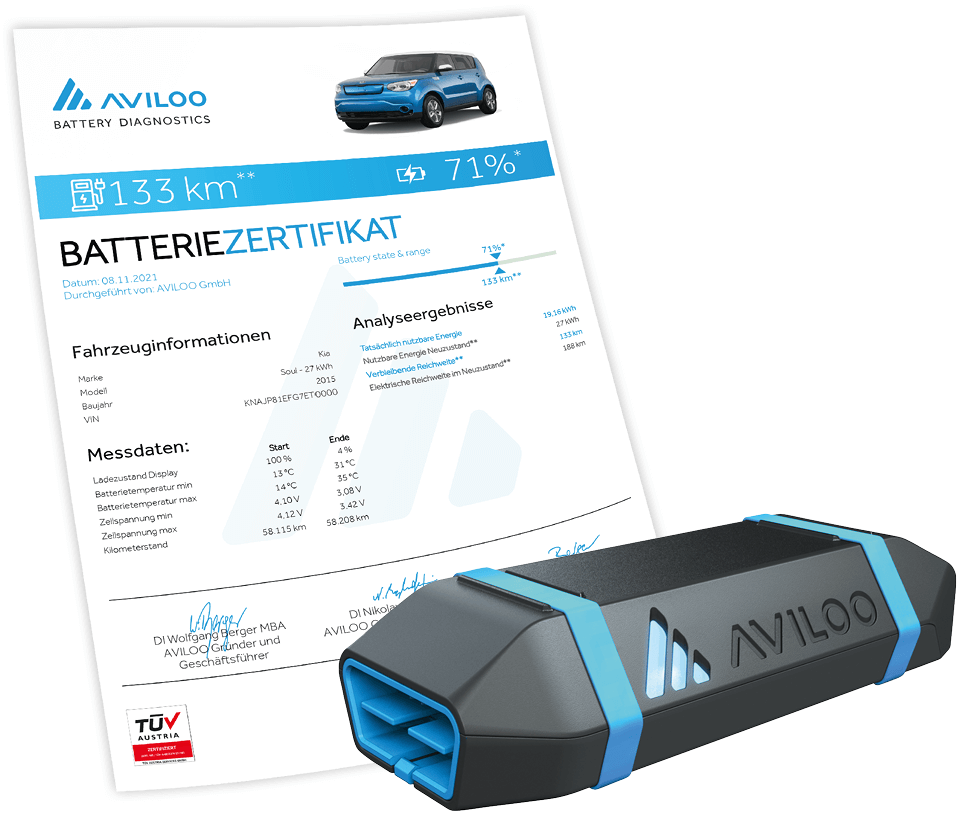
\includegraphics[width=0.9\textwidth]{images/aviloo_certificate.png}
%    \caption[AVILOO's battery test certificate and monitoring device]{AVILOO's battery test certificate and monitoring device. Taken from AVILOO's official website\footref{note:aviloo_website}.}
%    \label{fig:aviloo_certificate}
%\end{figure}

%The field data collected during each bcheck can be viewed on a portal called AVILOO Battery Cloud, and consists of measurements such as voltage, internal and external temperature, current, SOC, power consumption and so on, sampled with a relatively high frequency and possibly at the cell, module and pack level simultaneously. EV monitoring data is extremely useful in designing data-driven methods to predict the SOH of a battery pack, as discussed throughout this thesis.